\documentclass[aspectratio=169]{beamer}
\usepackage[T1]{fontenc}
\usepackage[utf8]{inputenc}
\usepackage{tikz}
\usepackage{graphicx}
\usepackage{listings}
\usepackage{xcolor}
\usepackage{hyperref}
\usepackage[spanish,es-noquoting]{babel}
\usepackage[round]{natbib}

\lstset{
  basicstyle=\ttfamily\small,
  keywordstyle=\color{blue},
  stringstyle=\color{red},
  commentstyle=\color{gray},
  showstringspaces=false
}

% Clean Theme Setup & Optimization
\usetheme{Warsaw}
\usecolortheme{default}
\usefonttheme{serif}

% Remove top headline bar and navigation clutter to maximize slide text space
\setbeamertemplate{headline}{}
\setbeamertemplate{navigation symbols}{}
\setbeamertemplate{frametitle continuation}{}

% Slim, clean footline bar
\setbeamertemplate{footline}{
  \leavevmode%
  \hbox{%
    \begin{beamercolorbox}[wd=.333333\paperwidth,ht=2.25ex,dp=1ex,left]{author in head/foot}%
      \hspace*{2ex}\insertshortauthor
    \end{beamercolorbox}%
    \begin{beamercolorbox}[wd=.333333\paperwidth,ht=2.25ex,dp=1ex,center]{title in head/foot}%
      \insertshorttitle
    \end{beamercolorbox}%
    \begin{beamercolorbox}[wd=.333333\paperwidth,ht=2.25ex,dp=1ex,right]{date in head/foot}%
      \insertframenumber{} / \inserttotalframenumber\hspace*{2ex}
    \end{beamercolorbox}%
  }%
  \vskip0pt%
}

% Font size and list spacing optimizations to prevent text overflow
\setbeamertemplate{itemize/enumerate body begin}{\small}
\setbeamertemplate{itemize/enumerate subbody begin}{\footnotesize}
\setbeamertemplate{itemize/enumerate subsubbody begin}{\scriptsize}

\makeatletter
\g@addto@macro\itemize{%
  \setlength{\itemsep}{2pt}%
  \setlength{\parsep}{1pt}%
  \setlength{\topsep}{2pt}%
  \setlength{\partopsep}{0pt}%
}
\makeatother

\graphicspath{{../}{./}}
\setbeamertemplate{caption}[numbered]

% Title info
\title[ Diseñando una  PromptLibrary ]{ Diseñando una  PromptLibrary Jurídica (Sesión 1)}
\subtitle{ De la destreza individual a la infraestructura institucional de la firma}
\author{Ricardo Reyes-Jimenez}
\institute{Universidad de La Sabana}
\date{\today}


% Background image for title slide
\usebackgroundtemplate{
  \tikz\node[opacity=0.3]{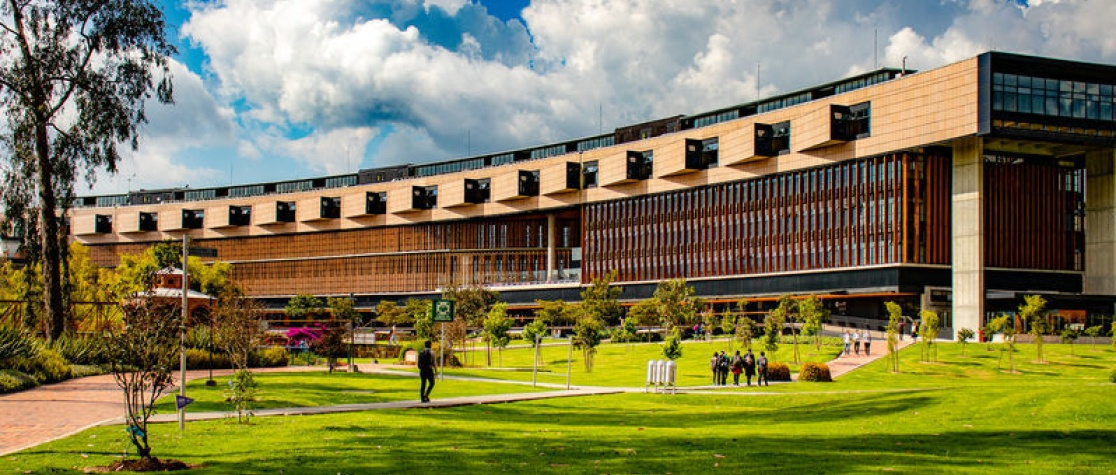
\includegraphics[width=\paperwidth,height=\paperheight]{Images/UniSabana.jpg}};
}


\begin{document}

% Title slide
\begin{frame}
  \titlepage
\end{frame}

% Reset background for normal slides
\usebackgroundtemplate{}


\begin{frame}[allowframebreaks,fragile]{Objetivos de la Sesión 1 (2 Horas)}

\begin{itemize}
  \item \textbf{Comprender la Paradoja de la IA Jurídica:} Por qué el aprendizaje aislado destruye valor en las organizaciones.
  \item \textbf{Dominar el concepto de PromptLibrary:} Repositorio centralizado de activos cognitivos reutilizables.
  \item \textbf{Aprender la anatomía del Blueprint Jurídico:} Estructura en 4 partes (Rol, Contexto, Variables y Restricciones).
  \item \textbf{Mapear casos de uso por especialidad:} Litigio, Derecho Corporativo/M\&A, Sector Público y Análisis Jurisprudencial.
  \item \textbf{Taller Práctico en Vivo:} Diseñar, documentar y ejecutar sus primeros Blueprints con pruebas de fuego.
  \item \textbf{Blindar la confidencialidad:} Gestión del secreto profesional y tratamiento de datos personales.
\end{itemize}
\end{frame}

\begin{frame}[allowframebreaks,fragile]{La Paradoja de la IA Jurídica}

\begin{itemize}
  \item Nunca ha sido tan accesible la Inteligencia  Artificial para el gremio legal.
  \item \textbf{Sin embargo:}
  \begin{itemize}
    \item Miles de horas de aprendizaje se evaporan a diario en conversaciones individuales.
    \item Los abogados trabajan en islas desconectadas.
    \item Los mejores prompts rara vez se documentan.
    \item Cada colega tropieza con las mismas piedras y reinventa la rueda.
  \end{itemize}
  \item \textbf{Diagnóstico:} El problema del sector legal hoy no es el acceso a la tecnología, sino la \textbf{ausencia de métodos para retener y escalar el conocimiento}.
\end{itemize}
\end{frame}

\begin{frame}[allowframebreaks,fragile]{El Costo Oculto de la Repetición Manual}

\begin{itemize}
  \item ¿Cuántas veces en un mes se realizan estas tareas en su despacho o entidad?
  \begin{itemize}
    \item Resúmenes ejecutivos de expedientes de 500 páginas.
    \item Cotejo de cláusulas de indemnidad y cambio de control.
    \item Elaboración de matrices de riesgos procesales o regulatorios.
    \item Búsqueda y contrastación de jurisprudencia reiterada.
    \item Proyección inicial de derechos de petición o recursos ordinarios.
  \end{itemize}
  \item \textbf{El costo real:} Cientos de horas mecánicas facturables que los clientes ya no quieren pagar o que retrasan el servicio judicial.
  \item \textbf{El riesgo:} Errores humanos inadvertidos por fatiga en tareas mecánicas.
\end{itemize}
\end{frame}

\begin{frame}[allowframebreaks,fragile]{El Problema de los ``Silos de Conocimiento''}

\begin{itemize}
  \item Un asociado junior invierte 45 minutos iterando hasta lograr que Gemini o Claude analice a la perfección un contrato de fideicomiso.
  \item El resultado es impecable. El asociado copia el texto, lo pega en Word, \textbf{cierra la pestaña del navegador} y continúa con su día.
  \item \textbf{¿Qué acaba de ocurrir?}
  \begin{itemize}
    \item Ese conocimiento (la instrucción exacta, las restricciones, el tono) se perdió en el éter.
    \item Mañana, otro asociado de la misma área empezará desde cero cometiendo los mismos fallos.
  \end{itemize}
  \item \textbf{La ceguera del prompt:} Creer que la victoria estuvo en el documento final, cuando el verdadero activo era la fórmula que lo generó.
\end{itemize}
\end{frame}

\begin{frame}[allowframebreaks,fragile]{¿Qué es una PromptLibrary Jurídica?}

\begin{itemize}
  \item \textbf{Definición Formal:} Un repositorio institucional organizado, probado, versionado y categorizado de instrucciones operativas (\textit{Blueprints}) listas para ser utilizadas por cualquier miembro del equipo.
  \item \textbf{No es una lista de ``trucos'' o ``hacks'' de internet.}
  \item \textbf{Es infraestructura de conocimiento:} La estandarización de cómo su organización le habla a la Inteligencia Artificial para producir entregables de alta calidad jurídica.
\end{itemize}
\end{frame}

\begin{frame}[allowframebreaks,fragile]{La Analogía del ``Banco de Minutas''}

\begin{itemize}
  \item En el ejercicio del Derecho, ninguna firma seria permite que cada abogado redacte un contrato de promesa de compraventa desde un archivo en blanco.
  \item \textbf{Toda firma u oficina jurídica posee:}
  \begin{itemize}
    \item Banco de minutas y contratos modelo.
    \item Formatos estándar de contestación de demandas.
    \item Guías de estilo y conceptos de referencia.
  \end{itemize}
  \item \textbf{La PromptLibrary es exactamente lo mismo:} El banco institucional de modelos, pero formulado para comunicarse con modelos de lenguaje masivos.
\end{itemize}
\end{frame}

\begin{frame}[allowframebreaks,fragile]{ROI Individual vs. ROI Institucional}

\begin{itemize}
  \item \textbf{Uso Individual:}
  \begin{itemize}
    \item 1 abogado ahorra 40 minutos en un concepto.
    \item Impacto: Marginal, personal y no transferible.
  \end{itemize}
  \item \textbf{Uso Institucional (PromptLibrary):}
  \begin{itemize}
    \item 50 abogados ahorran 40 minutos en cada concepto recurrente.
    \item El tiempo de ensayo y error se reduce de 45 minutos a 30 segundos.
    \item Se unifica el criterio de calidad y el tono institucional de la organización.
  \end{itemize}
  \item \textbf{Conclusión Estratégica:} El verdadero retorno de inversión (ROI) de la IA en el Derecho no está en la habilidad del individuo, sino en la \textbf{capacidad institucional de transferirla}.
\end{itemize}
\end{frame}

\begin{frame}[allowframebreaks,fragile]{Ciclo de Pérdida vs. Ciclo de Captura de Valor}

\begin{itemize}
  \item \textbf{El Ciclo de Pérdida (Estado Actual):}
  \begin{itemize}
    \item 1. Descubrimiento individual -> 2. Éxito puntual -> 3. Cierre de pestaña -> 4. Amnesia organizacional.
  \end{itemize}
  \item \textbf{El Ciclo de Captura (Con PromptLibrary):}
  \begin{itemize}
    \item 1. Descubrimiento -> 2. Parametrización en Blueprint -> 3. Prueba de estrés -> 4. Registro en el repositorio -> 5. Adopción colectiva inmediata.
  \end{itemize}
\end{itemize}
\end{frame}

\begin{frame}[allowframebreaks,fragile]{El Concepto de ``Blueprint'' (Plantilla Maestra)}

\begin{itemize}
  \item Un \textit{Blueprint} es un prompt parametrizado. No es un texto rígido para un solo cliente, sino un esqueleto reutilizable con campos variables.
  \item \textbf{Prompt Estático (Amateur - No reutilizable):}
  \begin{itemize}
    \item \textit{``Resume este contrato de arrendamiento del local comercial de la calle 72 para Juan Pérez.''}
  \end{itemize}
  \item \textbf{Blueprint Jurídico (Profesional - Reutilizable):}
  \begin{itemize}
    \item \textit{``Actúa como abogado senior especializado en \texttt{[ÁREA DEL DERECHO]}. Analiza el siguiente \texttt{[TIPO DE CONTRATO]}, representando los intereses de \texttt{[ROL DEL CLIENTE]}. Identifica las siguientes cláusulas críticas: \texttt{[LISTA DE ASPECTOS A REVISAR]}. Aplica las restricciones de \texttt{[JURISDICCIÓN]}. Texto: \texttt{[DOCUMENTO]}.''}
  \end{itemize}
\end{itemize}
\end{frame}

\begin{frame}[allowframebreaks,fragile]{Anatomía de un Blueprint Jurídico}

Todo Blueprint profesional debe contener al menos 4 elementos indispensables:
\begin{itemize}
  \item \textbf{Rol y Especialidad:} Define el nivel de pericia técnica y perspectiva (ej. \textit{Socio litigante laboral ante la Corte Suprema}).
  \item \textbf{Contexto Base:} Instrucciones inmutables sobre el objetivo del entregable, estructura esperada y tono.
  \item \textbf{Variables Clave (\texttt{[ ]}):} Campos delimitados entre corchetes para que el abogado usuario los complete en segundos.
  \item \textbf{Restricciones Infranqueables:} Lo que el modelo tiene estrictamente prohibido hacer (el dique contra alucinaciones).
\end{itemize}
\end{frame}

\begin{frame}[allowframebreaks,fragile]{El Poder de las Variables (El Secreto de los Corchetes)}

El uso sistemático de corchetes \texttt{[ ]} elimina la fricción para el usuario final:
\begin{itemize}
  \item \texttt{[TIPO DE DOCUMENTO]}: Contrato de obra / Demanda ordinaria / Pliego de condiciones.
  \item \texttt{[JURISDICCIÓN]}: Colombia (Código General del Proceso / Código Sustantivo del Trabajo).
  \item \texttt{[POSTURA DEL CLIENTE]}: Demandante / Convocante / Entidad pública contratante.
  \item \texttt{[PUNTOS DE DOLOR]}: Cláusulas penales, prescripción de la acción, vicios del consentimiento.
  \item \texttt{[TEXTO COMPLETO DEL EXPEDIENTE A PEGAR]}
\end{itemize}
\end{frame}

\begin{frame}[allowframebreaks,fragile]{Restricciones: El Componente Más Olvidado}

En derecho, la precisión radica en los límites que imponemos a la máquina:
\begin{itemize}
  \item \textbf{Anti-invención:} \textit{``Básate EXCLUSIVAMENTE en el texto anexo. Si un dato no figura expresamente, declara 'No hay información suficiente en el expediente'.''}
  \item \textbf{Fidelidad literal:} \textit{``Cita entre comillas las cláusulas pertinentes con su número respectivo.''}
  \item \textbf{Formato estructurado:} \textit{``Presenta los hallazgos en una tabla comparativa con 3 columnas: Cláusula, Riesgo Detectado, Recomendación de Ajuste.''}
  \item \textbf{Economía verbal:} \textit{``Omite fórmulas de cortesía, introducciones y justificaciones doctrinales no solicitadas.''}
\end{itemize}
\end{frame}

\begin{frame}[allowframebreaks,fragile]{Los 4 Errores Fatales al Diseñar Prompts Jurídicos}

\begin{itemize}
  \item \textbf{Ambigüedad Conceptual:} Pedir \textit{``revisar''} en vez de especificar el verbo técnico (\textit{``identificar contradicciones entre los testimonios A y B''}).
  \item \textbf{Falta de Contexto Fáctico:} Omitir la posición de parte del cliente o la naturaleza del proceso.
  \item \textbf{Ausencia de Restricciones Negativas:} No indicarle qué NO hacer, abriendo la puerta a prosa redundante o alucinaciones.
  \item \textbf{Objetivos Difusos:} Pretender resolver todo el litigio en una sola instrucción vaga.
\end{itemize}
\end{frame}

\begin{frame}[allowframebreaks,fragile]{Casos de Uso por Especialidad: Litigio}

\textbf{Blueprints de Alto Rendimiento para Litigantes:}
\begin{itemize}
  \item \textbf{Extracción de Cronologías Fácticas:} Mapeo temporal de hechos probados a partir de intercambios de correos o comunicaciones oficiales.
  \item \textbf{Detección de Contradicciones:} Cruce entre lo afirmado en la demanda, la contestación y las declaraciones testimoniales.
  \item \textbf{Esquematización de Contestación:} Identificación de excepciones de mérito y previas frente a cada pretensión.
  \item \textbf{Ficha de Riesgo Probatorio:} Evaluación de la conducencia, pertinencia y utilidad del material probatorio anexo.
\end{itemize}
\end{frame}

\begin{frame}[allowframebreaks,fragile]{Casos de Uso: Derecho Corporativo y M\&A}

\textbf{Blueprints para Transacciones y Asesoría Empresarial:}
\begin{itemize}
  \item \textbf{Auditoría Red-Flag en Data Rooms:} Detección de cláusulas de cambio de control, restricciones de cesión y exclusividades.
  \item \textbf{Memos Ejecutivos para Junta Directiva:} Síntesis de contingencias legales de 50 páginas en un resumen directivo de 2 páginas.
  \item \textbf{Revisión de Indemnidades y Límites de Responsabilidad:} Cotejo contra los estándares de negociación de la firma.
  \item \textbf{Traducción y Armonización Conceptual:} Adaptación de terminología de Common Law a instituciones del derecho civil local.
\end{itemize}
\end{frame}

\begin{frame}[allowframebreaks,fragile]{Casos de Uso: Sector Público y Contratación Estatal}

\textbf{Blueprints para Entidades y Asesores Estatales:}
\begin{itemize}
  \item \textbf{Cotejo de Requisitos Habilitantes:} Verificación rápida de cumplimiento de capacidad jurídica y financiera en ofertas complejas.
  \item \textbf{Respuestas Masivas a Derechos de Petición:} Clasificación de pretensiones ciudadanas y generación de borradores basados en la postura institucional.
  \item \textbf{Proyección de Actos Administrativos:} Estructuración metodológica de antecedentes fácticos y consideraciones jurídicas preliminares.
  \item \textbf{Matriz de Riesgos Contractuales:} Mapeo de tipologías de riesgo bajo los lineamientos de Colombia Compra Eficiente.
\end{itemize}
\end{frame}

\begin{frame}[allowframebreaks,fragile]{Casos de Uso: Análisis Jurisprudencial Sistemático}

\textbf{Ficha de Sentencia Estandarizada:}
\begin{itemize}
  \item \textbf{Objetivo:} Transformar un fallo judicial de 80 páginas en un activo de consulta rápida de 2 páginas.
  \item \textbf{Campos del Blueprint:}
  \begin{itemize}
    \item Tribunal, Sala, Magistrado Ponente y Fecha.
    \item Hechos jurídicamente relevantes depurados.
    \item Problema jurídico central formulado en pregunta.
    \item \textbf{Ratio Decidendi:} La regla de derecho vinculante creada o reiterada.
    \item \textbf{Obiter Dicta:} Consideraciones complementarias.
    \item Sentido de la decisión y salvamentos de voto.
  \end{itemize}
\end{itemize}
\end{frame}

\begin{frame}[allowframebreaks,fragile]{Herramientas para Empezar HOY (Fase 1: Mínima Fricción)}

\begin{itemize}
  \item \textbf{No compren software de miles de dólares para el Día 1.}
  \item La fricción tecnológica es la primera causa de muerte de la innovación en firmas legales.
  \item \textbf{Recomendación Práctica:} Empezar con un archivo compartido que todos usen ya (Excel en OneDrive, Google Sheets, Word Online o Notion).
  \item Lo determinante no es la plataforma informática: \textbf{es el rigor y la disciplina metodológica de documentar el Blueprint}.
\end{itemize}
\end{frame}

\begin{frame}[allowframebreaks,fragile]{Demo en Vivo: Estructura de la Versión 1.0}

\textit{(El Mentor proyecta una hoja de cálculo modelo)}
\begin{itemize}
  \item \textbf{Columna A:} Identificador y Nombre del Blueprint (ej. \textit{LIT-01: Cronología Procesal}).
  \item \textbf{Columna B:} Área de Práctica y Especialidad (\textit{Litigio Civil / Arbitraje}).
  \item \textbf{Columna C:} Objetivo Técnico del Entregable.
  \item \textbf{Columna D:} Texto del Blueprint (con variables en corchetes).
  \item \textbf{Columna E:} Modelo de IA Recomendado (ChatGPT, Claude 3.5 Sonnet, Gemini Pro).
  \item \textbf{Columna F:} Autor, Fecha y Versión (\textit{v1.0}).
  \item \textbf{Columna G:} Eficacia y Calificación del Equipo (1 a 5 estrellas).
\end{itemize}
\end{frame}

\begin{frame}[allowframebreaks,fragile]{Taller Práctico (Fase 1): Identificación (10 Minutos)}

\textbf{Trabajo en Mesas por Áreas de Práctica:}
\begin{itemize}
  \item Reúnanse con colegas de su misma especialidad (Litigio, Laboral, Corporativo, Público, etc.).
  \item Identifiquen \textbf{UNA} tarea repetitiva, mecánica y tediosa que realicen todas las semanas.
  \item Definan con absoluta precisión qué esperan obtener de la IA:
  \begin{itemize}
    \item ¿Cuál es el documento de entrada?
    \item ¿Cuál es el formato exacto del entregable final?
  \end{itemize}
\end{itemize}
\end{frame}

\begin{frame}[allowframebreaks,fragile]{Taller Práctico (Fase 2): Redacción del Blueprint (15 Minutos)}

\textbf{Elaboración de la Plantilla Maestra:}
\begin{itemize}
  \item Redacten el Blueprint en su documento colaborativo incorporando los 4 pilares:
  \begin{itemize}
    \item \textbf{Rol:} ¿A quién representa la IA?
    \item \textbf{Contexto:} ¿Cuál es la situación y normativa base?
    \item \textbf{Variables:} Usen \texttt{[ ]} para cada dato que cambie de caso en caso.
    \item \textbf{Restricciones:} Al menos 3 restricciones estrictas de formato, alucinación y tono.
  \end{itemize}
\end{itemize}
\end{frame}

\begin{frame}[allowframebreaks,fragile]{Taller Práctico (Fase 3): Prueba de Fuego (10 Minutos)}

\textbf{Ejecución y Stress-Testing en Vivo:}
\begin{itemize}
  \item Abran su plataforma de IA preferida (ChatGPT, Claude, Gemini).
  \item Copien su Blueprint, rellenen los corchetes con un caso real (previamente anonimizado) y envíen el prompt.
  \item \textbf{Preguntas de auditoría:}
  \begin{itemize}
    \item ¿El formato respetó lo solicitado?
    \item ¿El tono es acorde al estándar de su firma?
    \item ¿Qué faltó o qué sobró? Anoten el desvío para la Sesión 2.
  \end{itemize}
\end{itemize}
\end{frame}

\begin{frame}[allowframebreaks,fragile]{Blindaje Ético y Confidencialidad Jurídica}

\begin{itemize}
  \item \textbf{El Secreto Profesional (Art. 74 C.P.):} Es un deber deontológico inviolable.
  \item \textbf{Regla de Oro:} \textbf{NUNCA} peguen nombres de partes, números de cédula, contratos no públicos, secretos empresariales ni datos sensibles de clientes en herramientas de IA comerciales no corporativas.
  \item \textbf{Anonimización Previa:} Sustituyan partes por denominaciones genéricas: \texttt{[ARRENDADOR]}, \texttt{[EMPRESA A]}, \texttt{[TRABAJADOR X]}.
  \item \textbf{Protección de Datos Personales (Ley 1581 de 2012):} Asegurar que las políticas de privacidad de la herramienta cuenten con cláusulas de no-entrenamiento sobre los datos del usuario.
\end{itemize}
\end{frame}

\begin{frame}[allowframebreaks,fragile]{Criterio Profesional y Responsabilidad Jurídica}

\begin{itemize}
  \item \textbf{La IA es un asistente analítico de primer nivel; no es un abogado habilitado.}
  \item La responsabilidad profesional, disciplinaria y civil ante el cliente y el juez \textbf{recae siempre y exclusivamente sobre el abogado firmante}.
  \item Todo producto generado a través de un Blueprint debe someterse a:
  \begin{itemize}
    \item Verificación fáctica humana.
    \item Contrastación normativa de vigencia.
    \item Criterio estratégico final.
  \end{itemize}
\end{itemize}
\end{frame}

\begin{frame}[allowframebreaks,fragile]{Cierre de la Sesión 1 y Hoja de Ruta}

\begin{itemize}
  \item \textbf{Hito de Hoy:} Pasamos del conocimiento tácito y aislado a activos organizacionales documentados. Ya crearon su primer Blueprint institucional.
  \item \textbf{Para la Sesión 2 (Mañana):}
  \begin{itemize}
    \item Descubriremos por qué los prompts fallan y cómo refinarlos con técnicas Few-Shot.
    \item Aprenderemos a construir \textbf{Pipelines modulares} para procesos complejos.
    \item Analizaremos la hoja de ruta de escalabilidad y la \textbf{Gobernanza del Comité de IA}.
  \end{itemize}
  \item \textbf{¡Guarden sus Blueprints y los resultados de sus pruebas de fuego!}
\end{itemize}
\end{frame}




\end{document}